\documentclass[12pt]{article}
\usepackage[spanish]{babel}
\usepackage[utf8]{inputenc}
\usepackage{graphicx}
\usepackage{listings}
\usepackage{xcolor}
\usepackage{hyperref}
\usepackage{geometry}
\usepackage{caption}

\geometry{
    a4paper,
    top=2.5cm,
    bottom=2.5cm,
    left=3cm,
    right=3cm
}

\definecolor{codegreen}{rgb}{0,0.6,0}
\definecolor{codegray}{rgb}{0.5,0.5,0.5}
\definecolor{backcolour}{rgb}{0.95,0.95,0.95}

\lstdefinestyle{mystyle}{
    backgroundcolor=\color{backcolour},   
    commentstyle=\color{codegreen},
    keywordstyle=\color{blue},
    stringstyle=\color{codegreen},
    basicstyle=\ttfamily\small,
    breaklines=true,                 
    numbers=left,                    
    frame=single
}

\lstset{style=mystyle}

\begin{document}

\begin{titlepage}
    \begin{center}
        \vspace*{1cm}
        
\includegraphics{logo_uat}
        
        \vspace{2cm}
        {\huge\bfseries API RESTful para Sistemas Embebidos\par}
        \vspace{1cm}
        {\Large\itshape Documentación Técnica\par}
        
        \vspace{2cm}
        {\large\bfseries Integrantes del Equipo:\par}
        \vspace{0.5cm}
        {\large Juan Julián Paniagua Rico - a2213332303\par}
        {\large Isaac Sayeg Posadas Perez - a2213332197\par}
        {\large Jorge García Azua - matricula aqui\par}
        
        \vfill
        {\large Universidad Autonoma de Tamaulipas\par}
        {\large 8° Semestre - 2025\par}
    \end{center}
\end{titlepage}

\tableofcontents
\newpage

\section{Introducción}
Este proyecto implementa una API RESTful desarrollada en Node.js que permite la gestión de registros y decisiones para dispositivos embebidos. 

La solución integra una base de datos SQL Server para gestionar las tablas y procedimientos almacenados necesarios para sensores o actuadores. Este enfoque asegura la consolidación, consulta, y optimización de decisiones mediante algoritmos básicos embebidos.

\section{Estructura de la Base de Datos}
La base de datos se organiza en varias tablas y procedimientos almacenados. A continuación se detalla cada uno:

\subsection{Tablas}
La base de datos contiene las siguientes tablas principales utilizadas por la API:

\begin{itemize}
    \item \textbf{devices\_info:} Maneja la información básica de cada dispositivo.
    \begin{itemize}
        \item \textbf{id\_device:} Identificador único autoincremental.
        \item \textbf{id\_type:} Indica el tipo (sensor o actuador).
        \item \textbf{id\_signal\_type:} Relacionado al tipo de señal (digital o analógica).
        \item \textbf{name:} Nombre descriptivo del dispositivo.
        \item \textbf{vendor:} Fabricante del dispositivo.
    \end{itemize}
    
    \item \textbf{devices\_records:} Almacena los datos históricos de cada dispositivo.
    \begin{itemize}
        \item \textbf{id\_record:} Identificador único para cada lectura.
        \item \textbf{id\_device:} Relación con el dispositivo al que pertenece el registro.
        \item \textbf{current\_value:} Valor registrado.
        \item \textbf{date\_record:} Fecha y hora del registro.
    \end{itemize}
    
    \item \textbf{toma\_decisiones:} Contiene los datos para decisiones calculadas.
    \begin{itemize}
        \item \textbf{id\_decision:} Identificador único de decisión.
        \item \textbf{velocidad, distancia, decision:} Datos utilizados en el algoritmo.
        \item \textbf{date\_record:} Fecha y hora de la decisión.
    \end{itemize}
\end{itemize}

\subsection{Procedimientos Almacenados}
\noindent Los principales procedimientos almacenados implementados son:

\begin{enumerate}
    \item \textbf{SP\_Insert\_DevicesRecords:} Utilizado por la ruta POST para registrar el valor actual de un dispositivo.
    \begin{lstlisting}[language=SQL]
    CREATE PROCEDURE SP_Insert_DevicesRecords
        @id_device as numeric(18,0),
        @current_value as numeric(18,0)
    AS
    BEGIN
        INSERT INTO [devices_records]
            ([id_device], [date_record], [current_value])
        VALUES (@id_device, GETDATE(), @current_value)
    END
    \end{lstlisting}
    
    \item \textbf{SP\_SelectALL\_records:} Recupera todos los registros existentes en la tabla devices\_records.
    \begin{lstlisting}[language=SQL]
    CREATE PROCEDURE SP_SelectALL_records
    AS
    BEGIN
        SELECT DI.id_device, DI.name "NAME", 
               DR.current_value "CURRENT_VALUE", 
               DR.date_record "DATE_RECORD"
        FROM devices_records DR
        INNER JOIN devices_info DI 
            ON DR.id_device = DI.id_device
    END
    \end{lstlisting}
    
    \item \textbf{SP\_SelecLastDecision:} Recupera la última decisión registrada basada en las marcas de tiempo.
    \begin{lstlisting}[language=SQL]
    CREATE PROCEDURE SP_SelecLastDecision
    AS
    BEGIN
        SELECT TOP 1 *
        FROM toma_decisiones
        ORDER BY date_record DESC
    END
    \end{lstlisting}
\end{enumerate}

\section{Explicación del Código Backend}

\subsection{Punto de Entrada del Servidor}
El archivo \textbf{index.js} inicializa el servidor Express, configurando el API para escuchar en el puerto 3000. Además, gestiona la ruta raíz y da soporte a JSON.

\begin{lstlisting}[language=JavaScript]
const express = require('express');
const v1 = require('./v1/routes/Routes');

const app = express();
const PORT = process.env.PORT || 3000;

app.use(express.json());  // Habilita el soporte para JSON

// Configuración de rutas
app.use("/api/v1", v1);

app.get("/", (req, res) => {
    res.send("<h1>API RESTful en NodeJS para Servicios Embebidos</h1>")
});

// El servidor escucha en el puerto 3000
app.listen(PORT, () => {
    console.log(`Servidor escuchando en el puerto: ${PORT}`);
});
\end{lstlisting}

\subsection{Gestión de Rutas}
En \textbf{Routes.js}, las principales rutas a controlar son declaraciones GET y POST:

\begin{itemize}
    \item \textbf{GET /api/v1/} \\
    Devuelve registros al llamar al procedimiento almacenado SP\_SelectALL\_records:
    \begin{lstlisting}[language=JavaScript]
    router.get("/", controller.getAll_records);
    // getAll_records llama a los servicios y retorna los datos.
    \end{lstlisting}
    
    \item \textbf{POST /api/v1/registros} \\
    Inserta un registro nuevo utilizando el procedimiento SP\_Insert\_DevicesRecords:
    \begin{lstlisting}[language=JavaScript]
    router.post("/registros", controller.insertRecord);
    // El cuerpo debe incluir Id_device y Current_value.
    \end{lstlisting}
\end{itemize}

\subsection{Servicios}
El archivo \textbf{devicesService.js} implementa las funciones que conectan directamente con los procedimientos almacenados definidos:

\begin{lstlisting}[language=JavaScript]
const insertRecord = async function(JsonObj) {
    const id = JsonObj.Id_device;
    const current_value = JsonObj.Current_value;
    return await SP_Insert_DevicesRecords(id, current_value);
};
\end{lstlisting}

\section{Evidencia de Ejecución del Código}
A continuación, se presentan capturas de pantalla de la ejecución del código y las pruebas respectivas con la API:

\subsection{Servidor Express Configurado}
\begin{figure}[h!]
    \centering
    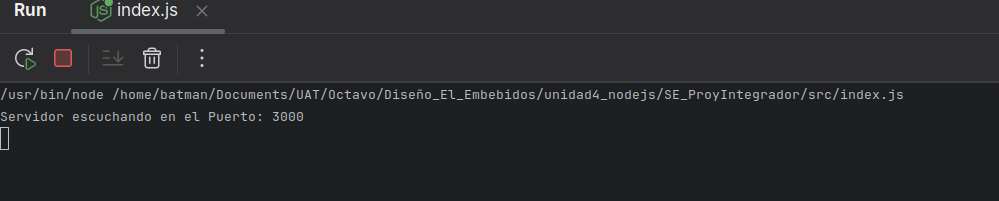
\includegraphics[width=0.8\textwidth]{server_running}
    \caption{Servidor Express ejecutándose correctamente en el puerto 3000.}
\end{figure}

\subsection{Prueba de Inserción en la Base de Datos}
\begin{figure}[h!]
    \centering
    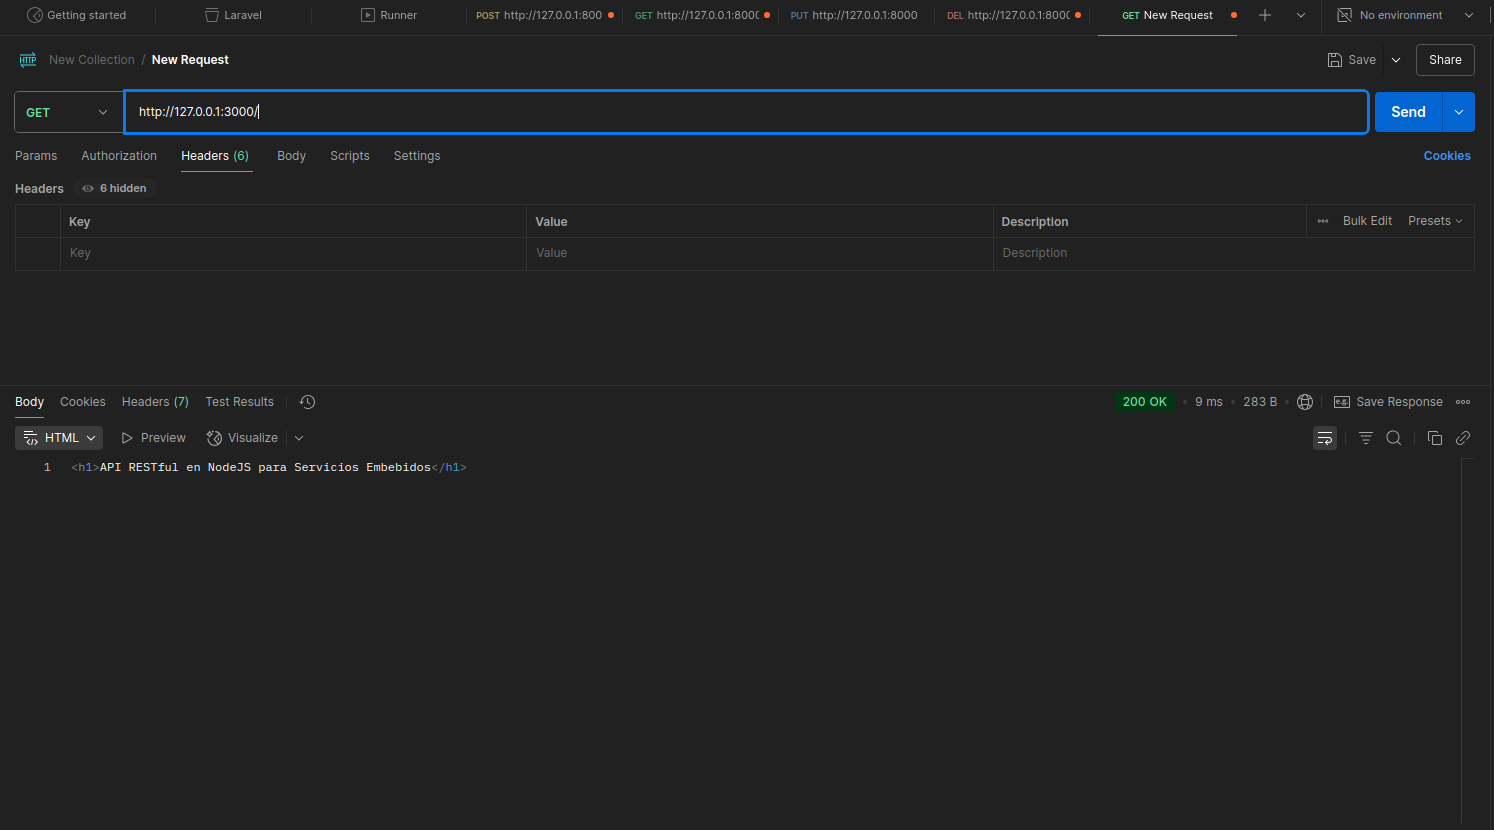
\includegraphics[width=0.8\textwidth]{postman_evidence}
    \caption{Prueba de registro nuevo utilizando el endpoint POST /api/v1/registros.}
\end{figure}

---

\end{document}